\chapter{Measuring compression: rate and distortion}\label{ch:measure}

\section{The four numbers}

\begin{description}
\item[Compression ratio] $=\dfrac{\text{raw bytes}}{\text{compressed bytes}}$. ``12:1'' means the file is a twelfth of the original. Higher is smaller.
\item[Bits per pixel (bpp)] $=\dfrac{8\cdot\text{compressed bytes}}{\text{number of pixels}}$. Raw is 8; this is the more convenient ``rate'' for plots because it does not depend on the picture size.
\item[MSE] (mean squared error) $=\dfrac{1}{N}\sum_{i}(\hat p_i-p_i)^2$ where $p_i$ are original and $\hat p_i$ reconstructed pixels. Squaring punishes large errors and makes everything positive.
\item[PSNR] (peak signal-to-noise ratio) $=10\log_{10}\dfrac{255^2}{\text{MSE}}$ decibels. It turns MSE into a number that grows as the picture gets better: 30\,dB is visibly degraded, 40\,dB is hard to tell apart, and every $+6$\,dB halves the typical pixel error (because it multiplies $255^2/\text{MSE}$ by 4).
\end{description}

\begin{warn}[Limits of PSNR]
PSNR is a pixel-by-pixel distance, not a model of human perception. Two images with the same PSNR can look very different (blurring versus blocky noise). Perception-based measures such as SSIM exist for this reason. PSNR remains the standard first number because it is simple, differentiable, and matches the maths of quantization noise.
\end{warn}

\section{The rate--distortion trade-off}

Every lossy codec lives on a curve: a lower rate costs a higher distortion. The ``quality'' slider just moves along that curve. A \emph{better codec} is one whose curve lies higher and further left (more PSNR for fewer bits).

\begin{figure}[h]
\centering
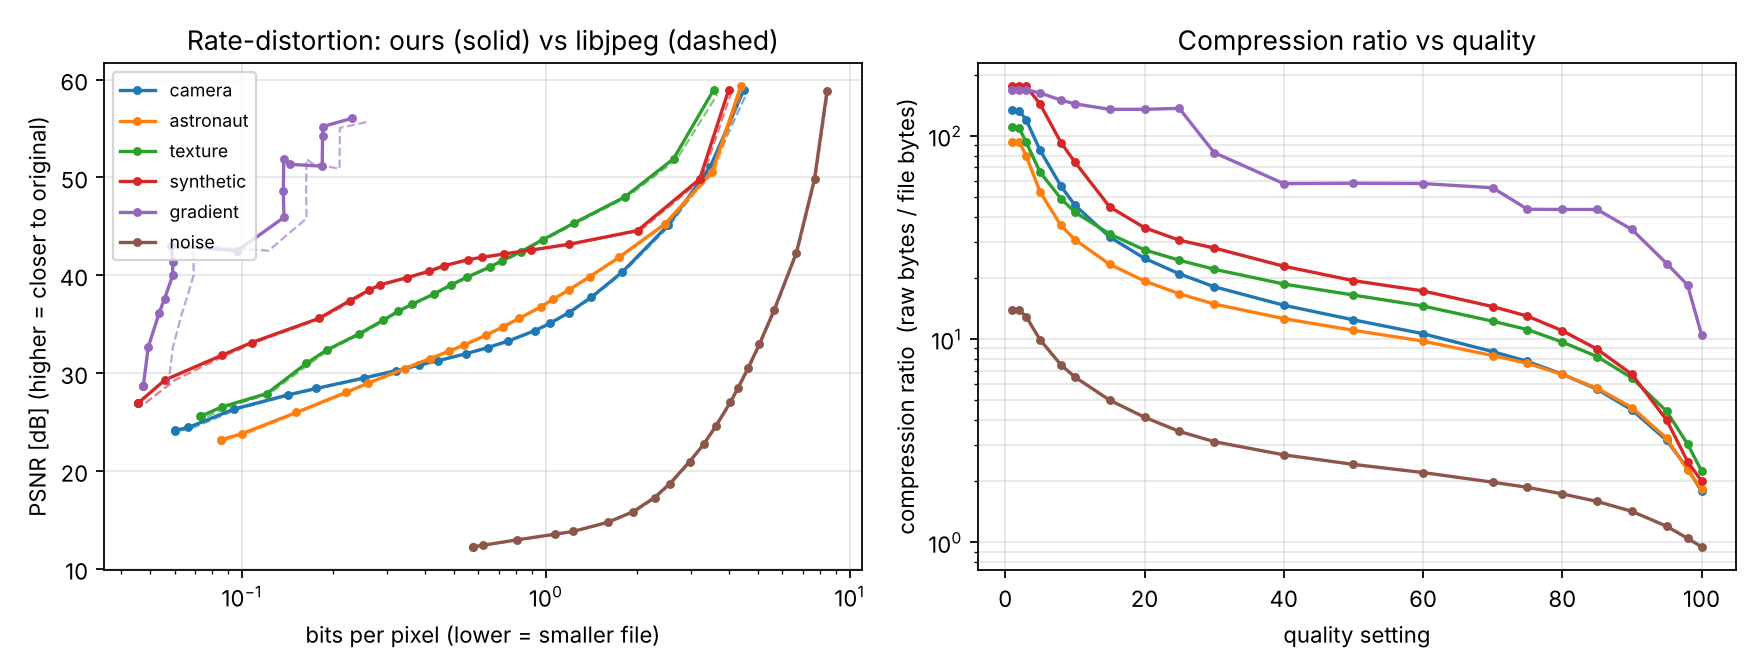
\includegraphics[width=\textwidth]{figures/rd_curves.png}
\caption{Left: PSNR versus bits per pixel for six test images (solid: this codec; dashed: libjpeg through Pillow, same quality values). Right: compression ratio versus quality setting.}
\end{figure}

\subsection{The cameraman in numbers}

\begin{center}
\small
\begin{tabular}{@{}rrrrrrr@{}}
\toprule
quality & bytes & bpp & ratio & MSE & PSNR [dB] & max error\\ \midrule
\inputrows{snippets/rd_camera}
\end{tabular}
\end{center}

How to read it:
\begin{itemize}
\item \textbf{Diminishing returns.} Going from quality 50 to 75 costs 1.6$\times$ the bytes and gains 2.5\,dB; going from 95 to 100 multiplies the file by 1.8 for $+14$\,dB that no human can see. The sweet spot for photographs is typically 75--90.
\item \textbf{Quality 100 is not lossless.} The step is 1 everywhere, so the only remaining error is rounding of coefficients (Chapter~\ref{ch:numerics}): MSE \camQhundredMSE, maximum error 1 grey level, and a file of 1.8:1.
\item \textbf{Quality 1 still gives something recognizable} at about 130:1, but it is dominated by blocks.
\end{itemize}

\subsection{What kind of picture compresses well?}

\begin{tabular}{@{}lp{12cm}@{}}
\toprule
\textbf{smooth gradient} & Almost all high-frequency coefficients are exactly zero already; at quality 50 the file is under 1.2 kB for 64 kB of pixels (more than 58:1).\\
\textbf{photographs} & Mixed smooth areas and edges: 8--20:1 is typical at quality 25--75.\\
\textbf{white noise} & Every pixel is independent, so no coefficient is small; quantization must throw away real information to save anything, PSNR collapses to about 23\,dB at quality 50, and at quality 100 the file is \emph{larger than the raw image} (ratio \noiseQhundredRatio). Compression only works on structured data.\\ \bottomrule
\end{tabular}

\begin{figure}[h]
\centering
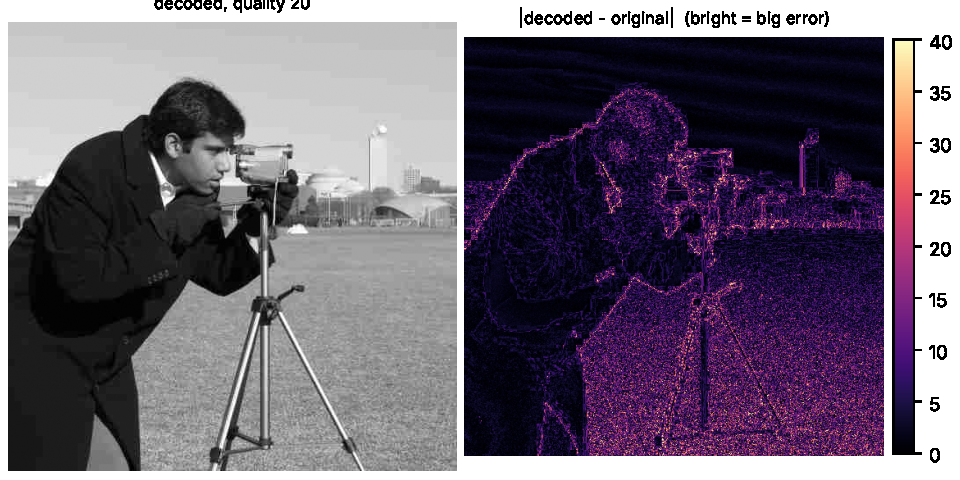
\includegraphics[width=0.78\textwidth]{figures/error_map.pdf}
\caption{Where the error is, at quality 20. It is largest on sharp edges (camera, tripod, skyline) and spread evenly over the fine texture of the grass, where many small high-frequency coefficients were rounded to zero. Smooth sky is nearly error-free.}
\end{figure}

\section{Sanity check against libjpeg}

How do we know our numbers are right and not merely self-consistent? Run the \emph{same} images through the reference implementation everybody uses, libjpeg (via the Pillow library), with the same quality values and optimized Huffman tables:

\begin{center}
\small
\begin{tabular}{@{}lrrrrr@{}}
\toprule
image & ours [B] & libjpeg [B] & difference & ours PSNR & libjpeg PSNR\\ \midrule
\inputrows{snippets/libjpeg_compare}
\end{tabular}
\end{center}

\begin{itemize}
\item \textbf{PSNR agrees to 0.01\,dB} on every image. That is strong evidence that our DCT, tables, quality scaling and rounding match the standard, because the distortion depends only on those.
\item \textbf{File sizes are within about 1\% on natural images} (ours slightly smaller). Sizes depend on the entropy coder and on container overhead, which legitimately differ: our header is smaller than JFIF plus marker segments, and we do not need byte stuffing. On near-constant images the fixed overhead dominates and the difference is larger (gradient). We are \emph{not} claiming to beat libjpeg; the comparison shows we are in the same league.
\item At quality 100 ours reaches slightly higher PSNR than libjpeg ($58.9$ vs $58.5$\,dB on the cameraman). A plausible reason is that libjpeg's default DCT is a fixed-point integer algorithm, and ours uses \texttt{double}; I did not isolate this, so say ``likely''.
\end{itemize}

\begin{sound}
``I swept quality from 1 to 100 on six images and plotted PSNR against bits per pixel. At each quality the PSNR matches libjpeg to 0.01\,dB and file sizes are within about 1\% on natural images, which validates the transform and quantization stages independently of my own tests. White noise is the worst case; a smooth gradient is the best case.''
\end{sound}
